\section{Analog-to-Digital Converter (ADC)}

\subsection{ADC Fundamentals}

\begin{concept}{ADC Overview}\\
An Analog-to-Digital Converter (ADC) converts continuous analog signals into discrete digital values:
\begin{itemize}
    \item Transforms analog voltage levels into corresponding digital values
    \item Resolution determined by number of bits (N)
    \item $2^N$ possible digital values (e.g., 12-bit ADC has 4096 levels)
    \item Converts real-world continuous signals (temperature, pressure, etc.) into digital form for processing
\end{itemize}
\end{concept}

\begin{definition}{ADC Terminology}\\
Key terms and concepts:
\begin{itemize}
    \item \textbf{Resolution}: Number of bits (N) in the digital output
    \item \textbf{LSB} (Least Significant Bit): Smallest detectable voltage change
    \begin{itemize}
        \item $LSB = \frac{V_{REF}}{2^N}$
    \end{itemize}
    \item \textbf{FSR} (Full Scale Range): Range between minimum and maximum digital codes
    \begin{itemize}
        \item $FSR = V_{REF} - 1 LSB$
    \end{itemize}
    \item \textbf{Sampling Rate}: Number of conversions per second
    \item \textbf{Conversion Time}: Time from start of sampling to digital output availability
    \item \textbf{Reference Voltage} ($V_{REF}$): Voltage that defines the ADC's full-scale range
\end{itemize}
\end{definition}

\begin{concept}{ADC Operating Principle}\\
\textbf{Flash ADC (Parallel ADC)}:
\begin{itemize}
    \item Uses comparators for each voltage level
    \item Input voltage compared to reference voltages simultaneously
    \item Fast but requires many components (e.g., 255 comparators for 8-bit)
\end{itemize}
\textbf{Successive Approximation Register (SAR) ADC}:
\begin{itemize}
    \item Uses binary search algorithm
    \item Compares input to successive approximations
    \item Takes N steps for N-bit resolution
    \item Good balance of speed, power, and complexity
    \item Most common in microcontrollers
\end{itemize}
\end{concept}

\subsection{ADC Errors and Characteristics}

\begin{definition}{Sampling Theorem}\\
According to the Nyquist-Shannon sampling theorem:
\begin{itemize}
    \item Sampling rate must be at least twice the highest frequency component of the input signal
    \item $f_{sampling} \geq 2 \times f_{max}$
    \item Prevents aliasing (false lower frequencies appearing in sampled signal)
\end{itemize}
\end{definition}

\begin{concept}{ADC Error Types}\\
\textbf{Quantization Error}:
\begin{itemize}
    \item Inherent error due to rounding analog values to discrete digital levels
    \item Range between -0.5 LSB and +0.5 LSB
    \item Cannot be eliminated, but reduced by increasing resolution
\end{itemize}
\textbf{Offset Error}:
\begin{itemize}
    \item Deviation from ideal ADC at zero input
    \item For ideal ADC, first transition occurs at 0.5 LSB
    \item Can be corrected through calibration
\end{itemize}
\textbf{Gain Error}:
\begin{itemize}
    \item Difference in slope between actual and ideal transfer function
    \item Expressed in LSB or as percentage of full-scale range (\%FSR)
    \item Can be corrected through calibration
\end{itemize}
\end{concept}

\begin{formula}{ADC Calculations}\\
\textbf{LSB Voltage}:
\begin{align}
V_{LSB} = \frac{V_{REF}}{2^N}
\end{align}

\textbf{Digital Output Value}:
\begin{align}
D_{out} = \frac{V_{in} \times 2^N}{V_{REF}}
\end{align}

\textbf{Analog Input from Digital Value}:
\begin{align}
V_{in} = \frac{D_{out} \times V_{REF}}{2^N}
\end{align}

\textbf{Percent Full Scale Range}:
\begin{align}
\%FSR = \frac{V_{in}}{V_{REF}} \times 100\%
\end{align}
\end{formula}

\subsection{STM32F4 ADC Features}

\begin{concept}{STM32F4 ADC Architecture}\\
The STM32F4 includes ADC modules with the following features:
\begin{itemize}
    \item Three ADCs (ADC1, ADC2, ADC3)
    \item 12-bit resolution (configurable to 10, 8, or 6 bits)
    \item Up to 24 external channels (16 on each ADC)
    \item Internal channels (temperature sensor, V$_{REFINT}$, V$_{BAT}$)
    \item Multiple operating modes:
    \begin{itemize}
        \item Single conversion vs. continuous conversion
        \item Single channel vs. scan mode (multiple channels)
    \end{itemize}
    \item Maximum sampling rate up to 2.4 MSPS (million samples per second)
    \item DMA capability
    \item Configurable sampling time
    \item Analog watchdog for threshold monitoring
\end{itemize}
\end{concept}

\begin{definition}{ADC Conversion Modes}\\
\textbf{Single vs. Continuous Conversion}:
\begin{itemize}
    \item \textbf{Single Conversion}: Performs one conversion, then stops
    \item \textbf{Continuous Conversion}: Continuously performs conversions without CPU intervention
\end{itemize}
\textbf{Single Channel vs. Scan Mode}:
\begin{itemize}
    \item \textbf{Single Channel}: Converts one channel only
    \item \textbf{Scan Mode}: Converts multiple channels in sequence
\end{itemize}
This results in four possible combinations:
\begin{itemize}
    \item Single channel, single conversion (simplest mode)
    \item Single channel, continuous conversion (monitor one input)
    \item Multi-channel, single conversion (read multiple inputs once)
    \item Multi-channel, continuous conversion (monitor multiple inputs)
\end{itemize}
\end{definition}

\subsection{STM32F4 ADC Configuration}

\begin{definition}{ADC Registers}\\
Key ADC registers on STM32F4:
\begin{itemize}
    \item \textbf{ADC\_SR}: Status register (flags for EOC, overrun, etc.)
    \item \textbf{ADC\_CR1}: Control register 1 (scan mode, resolution, etc.)
    \item \textbf{ADC\_CR2}: Control register 2 (conversion start, data alignment, etc.)
    \item \textbf{ADC\_SMPRx}: Sample time registers
    \item \textbf{ADC\_SQRx}: Regular sequence registers
    \item \textbf{ADC\_DR}: Data register (conversion result)
    \item \textbf{ADC\_CCR}: Common control register (for all ADCs)
\end{itemize}
\end{definition}

\begin{KR}{Basic ADC Configuration}
\paragraph{Step 1: Enable GPIO and ADC clocks}
Enable the clock to the GPIO port and ADC.
\paragraph{Step 2: Configure GPIO pins}
Configure the GPIO pins as analog inputs.
\paragraph{Step 3: Configure ADC parameters}
Set resolution, scan mode, conversion mode, and alignment.
\paragraph{Step 4: Configure channel and sampling time}
Set the channel sequence and sampling time.
\paragraph{Step 5: Enable ADC}
Turn on the ADC.

\begin{lstlisting}[language=C, style=basesmol]
// Configure ADC1 Channel 0 (PA0) for single conversion

// Step 1: Enable GPIO and ADC clocks
RCC->AHB1ENR |= RCC_AHB1ENR_GPIOAEN;  // Enable GPIOA clock
RCC->APB2ENR |= RCC_APB2ENR_ADC1EN;   // Enable ADC1 clock

// Step 2: Configure PA0 as analog input
GPIOA->MODER |= GPIO_MODER_MODER0;  // Analog mode (0b11)

// Step 3: Configure ADC parameters
// ADC Common Control Register
ADC->CCR &= ~ADC_CCR_ADCPRE;  // ADCPRE = 0 (APB2/2, typically 42MHz/2 = 21MHz)

// ADC1 Control Register 1
ADC1->CR1 &= ~ADC_CR1_RES;    // 12-bit resolution (default)
ADC1->CR1 &= ~ADC_CR1_SCAN;   // Disable scan mode (single channel)

// ADC1 Control Register 2
ADC1->CR2 &= ~ADC_CR2_CONT;   // Single conversion mode
ADC1->CR2 &= ~ADC_CR2_ALIGN;  // Right alignment
ADC1->CR2 &= ~ADC_CR2_EXTEN;  // Software trigger

// Step 4: Configure channel and sampling time
// Configure for channel 0
ADC1->SQR1 &= ~ADC_SQR1_L;     // 1 conversion in regular sequence
ADC1->SQR3 &= ~ADC_SQR3_SQ1;   // Clear channel selection
ADC1->SQR3 |= (0 << ADC_SQR3_SQ1_Pos);  // Channel 0 as first conversion

// Set sampling time for channel 0 (e.g., 84 cycles)
ADC1->SMPR2 &= ~ADC_SMPR2_SMP0;  // Clear bits
ADC1->SMPR2 |= (4 << ADC_SMPR2_SMP0_Pos);  // 84 cycles

// Step 5: Enable ADC
ADC1->CR2 |= ADC_CR2_ADON;  // Turn on ADC
\end{lstlisting}
\end{KR}

\begin{KR}{Performing ADC Conversion}
\paragraph{Start conversion}
Trigger the conversion using software or external trigger.
\paragraph{Wait for completion}
Check the EOC flag to determine when conversion is complete.
\paragraph{Read result}
Read the data register to get the conversion result.

\begin{lstlisting}[language=C, style=basesmol]
// Function to perform single ADC conversion
uint16_t ADC_ReadChannel(void) {
    // Start conversion
    ADC1->CR2 |= ADC_CR2_SWSTART;  // Software trigger to start conversion
    
    // Wait for conversion to complete
    while (!(ADC1->SR & ADC_SR_EOC)) { }
    
    // Read and return result
    return ADC1->DR;
}

// Function to convert ADC value to voltage
float ADC_ConvertToVoltage(uint16_t adcValue) {
    // Assuming VREF = 3.3V and 12-bit resolution (4096 levels)
    float voltage = (float)adcValue * 3.3f / 4095.0f;
    return voltage;
}
\end{lstlisting}
\end{KR}

\begin{KR}{Multi-Channel ADC Configuration}
\paragraph{Configure scan mode}
Enable scan mode to convert multiple channels.
\paragraph{Set up channel sequence}
Configure the sequence and number of channels.
\paragraph{Process results}
Read results for each channel in sequence.

\begin{lstlisting}[language=C, style=basesmol]
// Configure ADC for multi-channel scanning (channels 0, 1, and 4)

// Enable scan mode
ADC1->CR1 |= ADC_CR1_SCAN;

// Set number of conversions in sequence (3)
ADC1->SQR1 &= ~ADC_SQR1_L;
ADC1->SQR1 |= (2 << ADC_SQR1_L_Pos);  // L = 2 means 3 conversions

// Set channel sequence
ADC1->SQR3 = 0;  // Clear all
ADC1->SQR3 |= (0 << ADC_SQR3_SQ1_Pos);  // CH0 as 1st conversion
ADC1->SQR3 |= (1 << ADC_SQR3_SQ2_Pos);  // CH1 as 2nd conversion
ADC1->SQR3 |= (4 << ADC_SQR3_SQ3_Pos);  // CH4 as 3rd conversion

// Set sampling times for each channel
ADC1->SMPR2 &= ~(ADC_SMPR2_SMP0 | ADC_SMPR2_SMP1 | ADC_SMPR2_SMP4);
ADC1->SMPR2 |= (4 << ADC_SMPR2_SMP0_Pos);  // 84 cycles for CH0
ADC1->SMPR2 |= (4 << ADC_SMPR2_SMP1_Pos);  // 84 cycles for CH1
ADC1->SMPR2 |= (4 << ADC_SMPR2_SMP4_Pos);  // 84 cycles for CH4
\end{lstlisting}
\end{KR}

\begin{concept}{Analog Watchdog}\\
The Analog Watchdog monitors ADC conversion results against programmable thresholds:
\begin{itemize}
    \item Generates an interrupt if a conversion result is outside the threshold range
    \item Can be configured to monitor a single channel or all channels
    \item Useful for detecting abnormal voltage levels without CPU polling
    \item Programmable high and low thresholds
\end{itemize}
Applications:
\begin{itemize}
    \item Over-voltage/under-voltage detection
    \item Temperature limit monitoring
    \item Battery level monitoring
\end{itemize}
\end{concept}

\begin{KR}{Using DMA with ADC}
\paragraph{Configure DMA}
Set up DMA channel to transfer ADC results to memory.
\paragraph{Enable DMA for ADC}
Configure ADC to use DMA for data transfer.
\paragraph{Start conversion}
Start ADC conversion in continuous mode.

\begin{lstlisting}[language=C, style=basesmol]
// Configure ADC with DMA for continuous multi-channel sampling

// Configure DMA
RCC->AHB1ENR |= RCC_AHB1ENR_DMA2EN;  // Enable DMA2 clock

// Configure DMA2 Stream0 for ADC1
DMA2_Stream0->CR &= ~DMA_SxCR_EN;  // Disable DMA stream
while (DMA2_Stream0->CR & DMA_SxCR_EN) { }  // Wait until disabled

DMA2_Stream0->CR = 0;
DMA2_Stream0->CR |= (0 << DMA_SxCR_CHSEL_Pos);  // Channel 0
DMA2_Stream0->CR |= DMA_SxCR_PL_1;  // Priority high
DMA2_Stream0->CR |= DMA_SxCR_MSIZE_0;  // Memory data size: 16-bit
DMA2_Stream0->CR |= DMA_SxCR_PSIZE_0;  // Peripheral data size: 16-bit
DMA2_Stream0->CR |= DMA_SxCR_MINC;  // Memory increment mode
DMA2_Stream0->CR &= ~DMA_SxCR_PINC;  // Peripheral fixed
DMA2_Stream0->CR |= DMA_SxCR_CIRC;  // Circular mode

// Set addresses
DMA2_Stream0->PAR = (uint32_t)&ADC1->DR;  // Source: ADC1 data register
DMA2_Stream0->M0AR = (uint32_t)adc_values;  // Destination: buffer
DMA2_Stream0->NDTR = 3;  // Number of data items (3 channels)

// Enable DMA stream
DMA2_Stream0->CR |= DMA_SxCR_EN;

// Configure ADC for DMA
ADC1->CR2 |= ADC_CR2_DMA;  // Enable DMA mode
ADC1->CR2 |= ADC_CR2_CONT;  // Continuous conversion mode

// Start ADC conversion
ADC1->CR2 |= ADC_CR2_SWSTART;
\end{lstlisting}
\end{KR}

\begin{example2}{ADC Configuration Exercise}\\
Configure ADC1 to measure an analog voltage on pin PA5, with 12-bit resolution. Convert the result to a voltage between 0-3.3V.
\tcblower
1. Configure PA5 as an analog input
2. Configure ADC1 for 12-bit resolution, single conversion, single channel
3. Set appropriate sampling time
4. Perform conversion and convert result to voltage

\begin{lstlisting}[language=C, style=basesmol]
// Configure PA5 as analog input
RCC->AHB1ENR |= RCC_AHB1ENR_GPIOAEN;  // Enable GPIOA clock
RCC->APB2ENR |= RCC_PB2ENR_ADC1EN;   // Enable ADC1 clock
GPIOA->MODER |= GPIO_MODER_MODER5;    // Set PA5 to analog mode (0b11)

// Configure ADC1
ADC1->CR1 &= ~ADC_CR1_RES;     // 12-bit resolution (default)
ADC1->CR2 &= ~ADC_CR2_CONT;    // Single conversion mode
ADC1->CR2 &= ~ADC_CR2_ALIGN;   // Right alignment

// Configure for channel 5 (PA5)
ADC1->SQR1 &= ~ADC_SQR1_L;      // 1 conversion in sequence
ADC1->SQR3 &= ~ADC_SQR3_SQ1;    // Clear channel selection
ADC1->SQR3 |= (5 << ADC_SQR3_SQ1_Pos);  // Channel 5 as first conversion

// Set sampling time (84 cycles)
ADC1->SMPR2 &= ~ADC_SMPR2_SMP5;
ADC1->SMPR2 |= (4 << ADC_SMPR2_SMP5_Pos);

// Enable ADC
ADC1->CR2 |= ADC_CR2_ADON;

// Function to read ADC and convert to voltage
float ReadVoltage(void) {
    // Start conversion
    ADC1->CR2 |= ADC_CR2_SWSTART;
    
    // Wait for conversion to complete
    while (!(ADC1->SR & ADC_SR_EOC)) { }
    
    // Read ADC value
    uint16_t adcValue = ADC1->DR;
    
    // Convert to voltage (0-3.3V)
    float voltage = (float)adcValue * 3.3f / 4095.0f;
    
    return voltage;
}
\end{lstlisting}
\end{example2}

\section{ADC/DAC Exercises}

\important{SEP Handout Beilage ADC: addresses and configurations for ADC registers, Data Alignment}

\subsection{ADC Error Analysis}

\begin{KR}{Analyzing ADC Errors}
\paragraph{Understand error types}
\begin{itemize}
    \item \textbf{Quantization error:} Inherent error between -0.5 LSB and +0.5 LSB
    \item \textbf{Offset error:} Deviation from ideal transfer function at zero input
    \item \textbf{Gain error:} Deviation of the slope from ideal transfer function
    \item \textbf{Full-scale error:} Combination of offset and gain error at maximum input
\end{itemize}

\paragraph{Determine ADC resolution}
\begin{itemize}
    \item Calculate LSB size: LSB = V$_{REF}$ / 2$^N$ where N is the number of bits
    \item Example: 3-bit ADC with V$_{REF}$ = 2V has LSB = 2V/8 = 0.25V
\end{itemize}

\paragraph{Draw ideal transfer function}
\begin{itemize}
    \item Plot digital output vs. analog input
    \item First transition at 0.5 LSB
    \item Each subsequent transition at (i + 0.5) × LSB
    \item For N-bit ADC: 2$^N$ - 1 total steps
\end{itemize}

\paragraph{Calculate error values}
\begin{itemize}
    \item \textbf{Offset error in LSB:} Measure deviation at zero input
    \item \textbf{Offset error in volts:} Multiply LSB by offset error in LSB
    \item \textbf{Gain error in LSB:} Difference between actual and ideal slope
    \item \textbf{Error as percentage of FSR (\%FSR):} (Error in volts / FSR) × 100\%
    \begin{itemize}
        \item FSR (Full Scale Range) = V$_{REF}$ - 1 LSB
    \end{itemize}
\end{itemize}
\end{KR}

\begin{example2}{ADC Error Analysis}\\
For a 3-bit ADC with V$_{REF}$ = 2V and an offset error of -1.5 LSB:

\begin{enumerate}
    \item Draw the ideal transfer function
    \item Draw the actual transfer function with the offset error
    \item Calculate the LSB in volts
    \item Calculate the offset error in volts
    \item Calculate the offset error as a percentage of FSR
\end{enumerate}

\paragraph{Solution:}
1. \textbf{Ideal transfer function:}
\begin{itemize}
    \item N = 3 bits → 8 possible output codes (000 to 111)
    \item LSB = 2V/2$^3$ = 2V/8 = 0.25V
    \item First transition: 0.5 × LSB = 0.125V
    \item Code transitions at: 0.125V, 0.375V, 0.625V, 0.875V, 1.125V, 1.375V, 1.625V
\end{itemize}

2. \textbf{Actual transfer function with offset error:}
\begin{itemize}
    \item Offset error = -1.5 LSB
    \item All transitions shift by -1.5 × 0.25V = -0.375V
    \item New transitions at: -0.25V, 0V, 0.25V, 0.5V, 0.75V, 1V, 1.25V
\end{itemize}

3. \textbf{LSB in volts:}
\begin{itemize}
    \item LSB = V$_{REF}$/2$^N$ = 2V/8 = 0.25V
\end{itemize}

4. \textbf{Offset error in volts:}
\begin{itemize}
    \item Offset error = -1.5 LSB × 0.25V/LSB = -0.375V
\end{itemize}

5. \textbf{Offset error as percentage of FSR:}
\begin{itemize}
    \item FSR = V$_{REF}$ - 1 LSB = 2V - 0.25V = 1.75V
    \item Offset error (\%FSR) = (-0.375V / 1.75V) × 100\% = -21.43\%
\end{itemize}
\end{example2}

\subsection{ADC Programming}

\begin{KR}{Configuring and Using STM32 ADCs}
\paragraph{Enable peripheral clocks}
\begin{itemize}
    \item Enable GPIO clock for analog pin
    \item Enable ADC clock in RCC register
\end{itemize}

\paragraph{Configure GPIO pin for analog mode}
\begin{itemize}
    \item Set GPIO MODE register bits to analog mode (11)
\end{itemize}

\paragraph{Configure ADC common settings}
\begin{itemize}
    \item Configure ADC clock prescaler in ADC\_CCR
    \item Enable/disable temperature sensor and internal reference
\end{itemize}

\paragraph{Configure ADC specific settings}
\begin{itemize}
    \item Set resolution in ADC\_CR1 (RES bits)
    \item Configure scan mode if using multiple channels
    \item Set conversion mode in ADC\_CR2 (CONT bit):
    \begin{itemize}
        \item 0: Single conversion
        \item 1: Continuous conversion
    \end{itemize}
    \item Set data alignment in ADC\_CR2 (ALIGN bit)
    \item Configure ADC trigger source if needed
\end{itemize}

\paragraph{Configure channel settings}
\begin{itemize}
    \item Set sampling time in ADC\_SMPR1/2 registers
    \item Configure regular sequence in ADC\_SQR1/2/3:
    \begin{itemize}
        \item Set sequence length in L[3:0] bits
        \item Set channel order in SQx[4:0] bits
    \end{itemize}
\end{itemize}

\paragraph{Start conversion and read results}
\begin{itemize}
    \item Enable ADC by setting ADON bit in ADC\_CR2
    \item Start conversion by setting SWSTART bit in ADC\_CR2
    \item Poll EOC flag in ADC\_SR or use interrupt
    \item Read conversion result from ADC\_DR
\end{itemize}
\end{KR}

\begin{example2}{ADC Configuration and Usage}\\
Write C code to configure and use ADC1 to read from channel 5 with 12-bit resolution in single conversion mode. The code should:

\begin{enumerate}
    \item Wait until ADC1 conversion has completed
    \item Set an 8-bit variable (var2) to 0xFF if there was a loss of data on ADC2, otherwise reset that variable to 0
    \item Set ADC3 resolution to 10-bit
\end{enumerate}

Use register addresses from the provided documentation.

\paragraph{Solution:}
First, let's define the relevant register addresses:
\begin{lstlisting}[language=C, style=basesmol]
// ADC1 registers
#define ADC1_SR     (*((volatile uint32_t*)(0x40012000)))  // Status register
#define ADC1_CR1    (*((volatile uint32_t*)(0x40012004)))  // Control register 1
#define ADC1_CR2    (*((volatile uint32_t*)(0x40012008)))  // Control register 2
#define ADC1_DR     (*((volatile uint32_t*)(0x4001204C)))  // Data register

// ADC2 registers
#define ADC2_SR     (*((volatile uint32_t*)(0x40012100)))  // Status register

// ADC3 registers
#define ADC3_CR1    (*((volatile uint32_t*)(0x40012204)))  // Control register 1

// Bit positions
#define ADC_SR_EOC  (1 << 1)  // End of conversion flag
#define ADC_SR_OVR  (1 << 5)  // Overrun flag
#define ADC_CR1_RES_MASK (3 << 24)  // Resolution mask
#define ADC_CR1_RES_10BIT (1 << 24)  // 10-bit resolution
\end{lstlisting}

Now, let's solve each part of the problem:

1. \textbf{Wait until ADC1 conversion has completed}
\begin{lstlisting}[language=C, style=basesmol]
// Wait for end of conversion flag
while (!(ADC1_SR & ADC_SR_EOC)) {
    // Empty loop
}
\end{lstlisting}

2. \textbf{Check for overrun on ADC2 and set var2 accordingly}
\begin{lstlisting}[language=C, style=basesmol]
uint8_t var2;
if (ADC2_SR & ADC_SR_OVR) {
    var2 = 0xFF;  // Overrun occurred
} else {
    var2 = 0x00;  // No overrun
}
\end{lstlisting}

3. \textbf{Set ADC3 resolution to 10-bit}
\begin{lstlisting}[language=C, style=basesmol]
// Clear resolution bits and set to 10-bit
ADC3_CR1 &= ~ADC_CR1_RES_MASK;  // Clear bits
ADC3_CR1 |= ADC_CR1_RES_10BIT;  // Set 10-bit resolution
\end{lstlisting}
\end{example2}

\begin{example2}{ADC Configuration and Usage (continued)}\\
Complete function:
\begin{lstlisting}[language=C, style=basesmol]
void adc_operations(void) {
    // 1. Wait until ADC1 conversion has completed
    while (!(ADC1_SR & ADC_SR_EOC)) {
        // Empty loop
    }
    
    // 2. Check for overrun on ADC2
    uint8_t var2;
    if (ADC2_SR & ADC_SR_OVR) {
        var2 = 0xFF;  // Overrun occurred
    } else {
        var2 = 0x00;  // No overrun
    }
    
    // 3. Set ADC3 resolution to 10-bit
    ADC3_CR1 &= ~ADC_CR1_RES_MASK;  // Clear bits
    ADC3_CR1 |= ADC_CR1_RES_10BIT;  // Set 10-bit resolution
}
\end{lstlisting}
\end{example2}

\section{ADC (Analog-Digital Converter)}

\subsection{ADC-Charakteristika und Fehler}

\begin{KR}{ADC Timing Diagramm}\\
    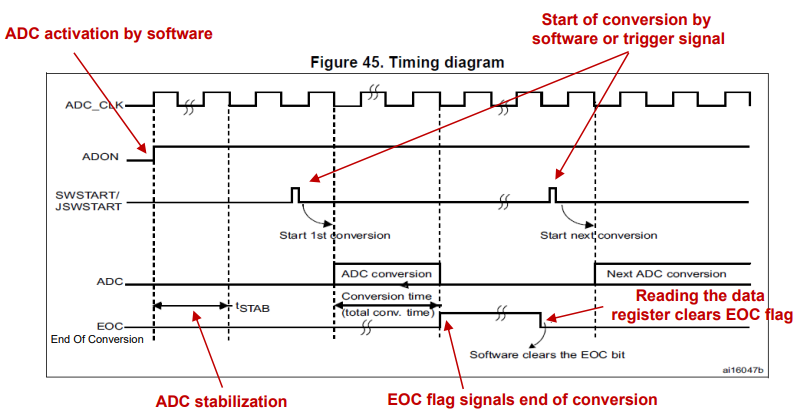
\includegraphics[width=\linewidth]{adc_timing_diagram.png}
\end{KR}

\begin{concept}{Fast Conversion Mode}\\
    It is possible to perform faster conversion by reducing the ADC resolution. The RES bits are used to select the number of bits available in the data register. The minimum conversion time for each resolution is then as follows:
- 12 bits: $3+12=15$ ADCCLK cycles
- 10 bits: $3+10=13$ ADCCLK cycles
- 8 bits: $3+8=11$ ADCCLK cycles
- 6 bits: $3+6=9$ ADCCLK cycles
\end{concept}

\begin{KR}{ADC Interrupts}\\
    An interrupt can be produced on the end of conversion for regular and injected groups, when the analog watchdog status bit is set and when the overrun status bit is set. Separate interrupt enable bits are available for flexibility.
Two other flags are present in the ADC\_SR register, but there is no interrupt associated with them:
- JSTRT (Start of conversion for channels of an injected group)
- STRT (Start of conversion for channels of a regular group)

Table 70. ADC interrupts
\begin{tabular}{|l|c|c|}
\hline \multicolumn{1}{|c|}{ Interrupt event } & Event flag & Enable control bit \\
\hline End of conversion of a regular group & EOC & EOCIE \\
\hline End of conversion of an injected group & JEOC & JEOCIE \\
\hline Analog watchdog status bit is set & AWD & AWDIE \\
\hline Overrun & OVR & OVRIE \\
\hline
\end{tabular}
\end{KR}

\important{SEP Handout Beilage ADC control register!!}

\begin{KR}{ADC Transfer-Funktion und Offset-Fehler}\\
    \paragraph{Grundlagen}
    \begin{itemize}
        \item LSB = V\_REF / $2^n$ (n = Anzahl Bits)
        \item FSR (Full Scale Range) = V\_REF - 1 LSB
        \item Idealer ADC: erste Transition bei 0.5 LSB
    \end{itemize}
    
    \paragraph{Offset-Fehler}
    \begin{itemize}
        \item Definition: Abweichung bei Eingangsspannung = 0V
        \item Messung: Zero-Scale-Spannung bis erste Transition
        \item Berechnung: Offset\_Error = gemessene\_Transition - 0.5 LSB
    \end{itemize}
    
    \paragraph{Fehler in Prozent FSR}
    \begin{itemize}
        \item Offset\_Error (\%FSR) = (Offset\_Error\_V $\times$ 100) / FSR\_V
        \item FSR\_V = V\_REF - 1 LSB
    \end{itemize}
    
    \paragraph{Transfer-Funktion zeichnen}
    \begin{enumerate}
        \item Zeichne ideale Treppenfunktion
        \item Verschiebe um Offset-Fehler (positiv = rechts, negativ = links)
        \item Erste Transition: 0.5 LSB + Offset\_Error
    \end{enumerate}
\end{KR}

\begin{example2}{3-Bit ADC mit Offset-Fehler}\\
    Idealer 3-Bit ADC mit V\_REF = 2V, Offset-Fehler = -1.5 LSB
    
    \tcblower

    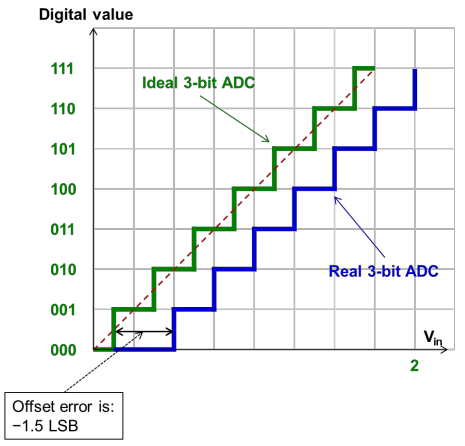
\includegraphics[width=\linewidth]{adc_offset_ex.png}
    
    \textbf{Berechnungen:}
    \begin{itemize}
        \item 1 LSB = 2V / $2^3$ = 2V / 8 = 0.25V
        \item Offset-Fehler = -1.5 $\times$ 0.25V = -0.375V
        \item FSR = 2V - 0.25V = 1.75V
        \item Offset-Fehler (\%FSR) = 0.375V $\times$ 100 / 1.75V = 21.43\%
    \end{itemize}
    
    \textbf{Transfer-Funktion:}
    \begin{itemize}
        \item Ideale erste Transition: 0.5 LSB = 0.125V
        \item Reale erste Transition: 0.125V - 0.375V = -0.25V
        \item Gesamte Kurve um 1.5 LSB nach links verschoben
    \end{itemize}
    
    \textbf{Digitale Werte:}
    Real-ADC erreicht digitalen Wert 001 bereits bei negativer Eingangsspannung, während ideal-ADC erst bei 0.125V den Wert 001 erreichen würde.
\end{example2}

\begin{example2}{ADC Positive Offset Error} In case of a positive offset error of +1.5 LSB, the graph will look like this:\\
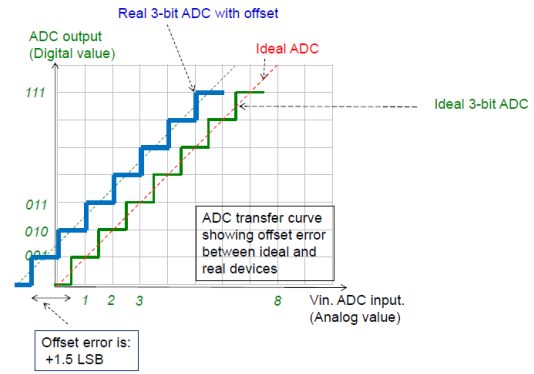
\includegraphics[width=\linewidth]{adc_positive_offset.png}
\end{example2}

\subsection{ADC-Programmierung STM32}

\begin{KR}{ADC-Register programmieren}\\
    \paragraph{Status-Register auswerten}
    \begin{itemize}
        \item EOC (End of Conversion): Bit 1 in ADC\_SR
        \item OVR (Overrun): Bit 5 in ADC\_SR
        \item Warten auf Conversion: \texttt{while (!(ADC\_SR \& 0x02))}
        \item Overrun prüfen: \texttt{if (ADC\_SR \& 0x20)}
    \end{itemize}
    
    \paragraph{Auflösung konfigurieren}
    \begin{itemize}
        \item RES[1:0] in ADC\_CR1 Register (Bits 25:24)
        \item 00: 12-bit, 01: 10-bit, 10: 8-bit, 11: 6-bit
        \item Einzelne Bits setzen/löschen mit Bit-Masken
    \end{itemize}
    
    \paragraph{Adressen berechnen}
    \begin{itemize}
        \item ADC1: 0x40012000 + Register\_Offset
        \item ADC2: 0x40012100 + Register\_Offset  
        \item ADC3: 0x40012200 + Register\_Offset
        \item Siehe Reference Manual für genaue Offsets
    \end{itemize}
    
    \paragraph{Bit-Manipulation}
    \begin{itemize}
        \item Bit setzen: \texttt{REG |= (1 << bit\_nr)}
        \item Bit löschen: \texttt{REG \&= \~{}(1 << bit\_nr)}
        \item Mehrere Bits: erst löschen, dann setzen
    \end{itemize}
\end{KR}

\begin{example2}{ADC-Programmierung Aufgaben}\\
    ADCs sind korrekt initialisiert. Schreibe C-Code für:
    \begin{enumerate}
        \item Warten bis ADC1 Conversion fertig
        \item Variable auf 0xFF setzen bei ADC2 Datenverlust
        \item ADC3 Auflösung auf 10-bit setzen
    \end{enumerate}
    
    \tcblower
    
    \textbf{Lösungen:}
    
    \textbf{a) Warten auf ADC1 EOC (Bit 1):}
\begin{lstlisting}[style=basesmol]
#define ADC1_SR (*((volatile uint32_t *)(0x40012000)))
while (!(ADC1_SR & 0x02)) {
    // Warten bis EOC gesetzt
}
\end{lstlisting}
Addresse des ADC1 Status-Registers ist 0x40012000 + base offset of ADC1 + status reg offset = 0x40012000
\vspace{2mm}\\

    \textbf{b) ADC2 Overrun prüfen (Bit 5):}
\begin{lstlisting}[style=basesmol]
#define ADC2_SR (*((volatile uint32_t *)(0x40012100)))
uint8_t var2;
if (ADC2_SR & 0x20) {
    var2 = 0xFF;  // Overrun aufgetreten
} else {
    var2 = 0x00;  // Kein Overrun
}
\end{lstlisting}
Addresse des ADC2 Status-Registers ist 0x40012000 + base offset of ADC2 + status reg offset = 0x40012100
\vspace{2mm}\\

    \textbf{c) ADC3 auf 10-bit (RES[25:24] = 01):}
\begin{lstlisting}[style=basesmol]
#define ADC3_CR1 (*((volatile uint32_t *)(0x40012204)))
ADC3_CR1 &= 0xFCFFFFFF;  // Bits 25:24 loeschen
ADC3_CR1 |= 0x01000000;  // Bit 24 setzen (01)

// kann auch so geschrieben werden:
ADC3_CR1 |= 0x01000000;  // force bit24 to 1
ADC3_CR1 &= 0xFDFFFFFF;  // force bit25 to 0
\end{lstlisting}
Addresse des ADC3 Status-Registers ist 0x40012000 + base offset of ADC3 + control reg1 offset = 0x40012204
\end{example2}

\begin{remark}
    Bei ADC-Registern ist es wichtig, die korrekten Bit-Positionen zu verwenden. EOC ist Bit 1 (nicht Bit 0), OVR ist Bit 5. Die Auflösung wird durch zwei Bits (RES[1:0]) in Bits 25:24 des CR1-Registers gesteuert.
\end{remark}